\section{ROS-people}
The ros-people package is a set of different ROS nodes that includes algorithms for detection of different parts of humans. These nodes can be connected and used for determination of a person's position in 3D space.\\

\subsection{Facial feature detection} \label{sec:Face}%detection 

To ensure detection of humans, multiple sensors will be used. One of these sensors is a camera that captures images in the average height of human faces to determine the presence of a person.\\

Calculating facial features can be computationally heavy due to the fact that many different features can be found on human faces. As the computer only perceives a face as a collection of pixels with different colour and/or light intensities it can be hard to detect a face, as shapes and sizes vary between different people.\\

To aid in the detection of faces, Paul Viola and Michael Jones created an optimisation algorithm, that utilises the Haar Classifier, that helps to quickly detect faces and other objects based on features known as Haar-like features\cite{Viola01robustreal-time}. These features use the change in contrast in rectangular groups of pixels to determine the relative dark and light areas of an object. A Haar-like feature contains two or three of these groups of relative contrast. The size of the examined pixel group can be increased or decreased in order to detect objects of different sizes. Different Haar-like features can be seen in figure \ref{fig:Haar-like}.

\begin{figure}[H]
    \centering
    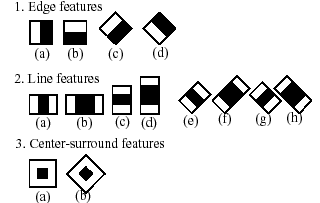
\includegraphics[width=.6\textwidth]{figures/CommonHaarFeatures.png}
    \caption{Common Haar-like features that can be used to determine if an image contains a persons face.\cite{wilson2006facial}}
    \label{fig:Haar-like}
\end{figure}

Due to the vast amount of faces needed to train a facial detection program using a Haar Classifier, OpenCV trained libraries has been used for this project. These libraries have been trained on 10,000 images of faces of over 1,000 people along with 5,000 images of non facial images.\cite{wilson2006facial}\\

\subsection{Source Code}
The software for face detection can be found in appendix \ref{}.\\
The overview of the main code can be reviewed in the flowchart below, see figure \ref{fig:flowchartFaceMain}.
\begin{figure}[H]
    \centering
    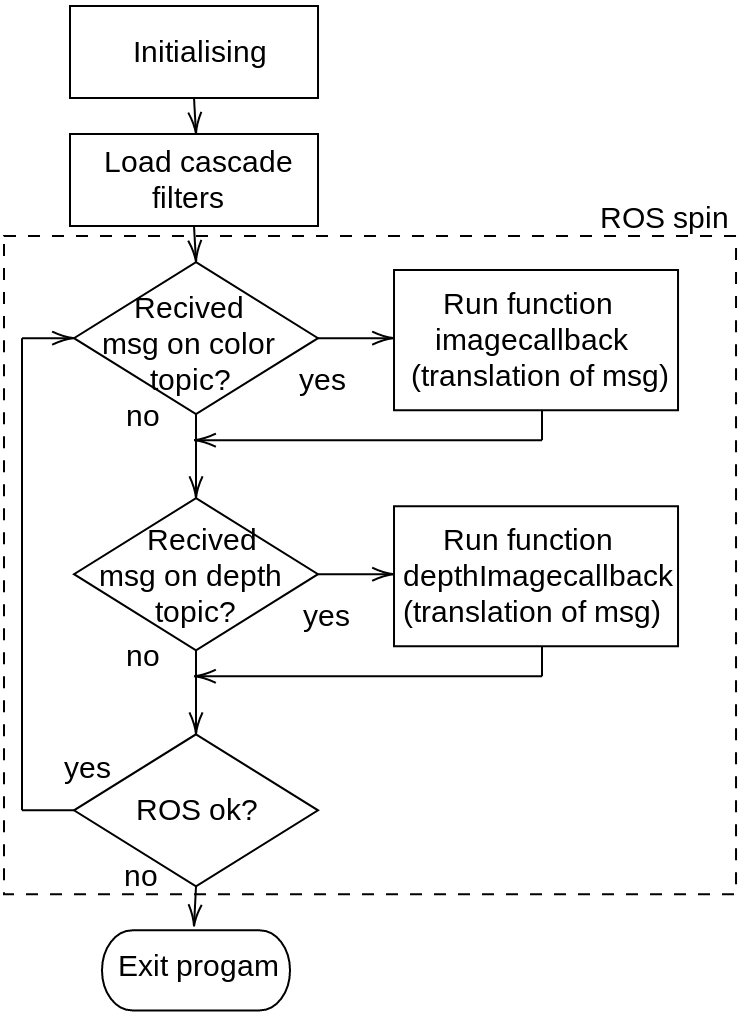
\includegraphics[width=0.5\textwidth]{figures/main_face_flow.png}
    \caption{Flowchart of main loop of the face detection, that are implemented in this project. One important step in this flow chart is the loading of the cascade filters. The primary functions are the callbacks imagecallback() and depthimagecallback(), this is where the ROS message gets  converted to an image for use in openCV.}
    \label{fig:flowchartFaceMain}
\end{figure}

The face detector takes in a stream of images and depth images from the Intel Real Sense camera on the robot. This is done in two callback functions called in the function \texttt{faceDetector()}. The callback for the depth images is used to calculate the depth of the face if one is found. The callback of the image starts the procedure of detecting a face in the image by calling the function \texttt{detectAndDisplay()}.\\

The function \texttt{detectAndDisplay()} is the primary function for the face detection of this project, see figure \ref{fig:flowchartDetectface}.
This function takes the image from the camera and detects a face if one is present and combines the location of the face with the distance from the face to be transmitted to the tracking node.

To do this, \texttt{detectAndDisplay()} first converts the image from the camera to grey scale, due to the fact that the function detectMultiScale, which is utilised to detect faces and eyes only, works on a grey scaled image. To improve the detection speed of the function, the images are scaled down to have fewer calculations for every image. The ratio between width and height of the image is kept in order to ensure the shape of the faces.\\

With the scaled image, histogram equalisation is performed. This operation helps ensure similar looking faces in any lighting condition, to prevent faces from not being detected due to poor lighting. This is done by stretching out the histogram to make the captured image lighter and as seen figure \ref{fig:contrast}, then the features of the face can be seen more easily.
\begin{figure}[H]
    \centering
    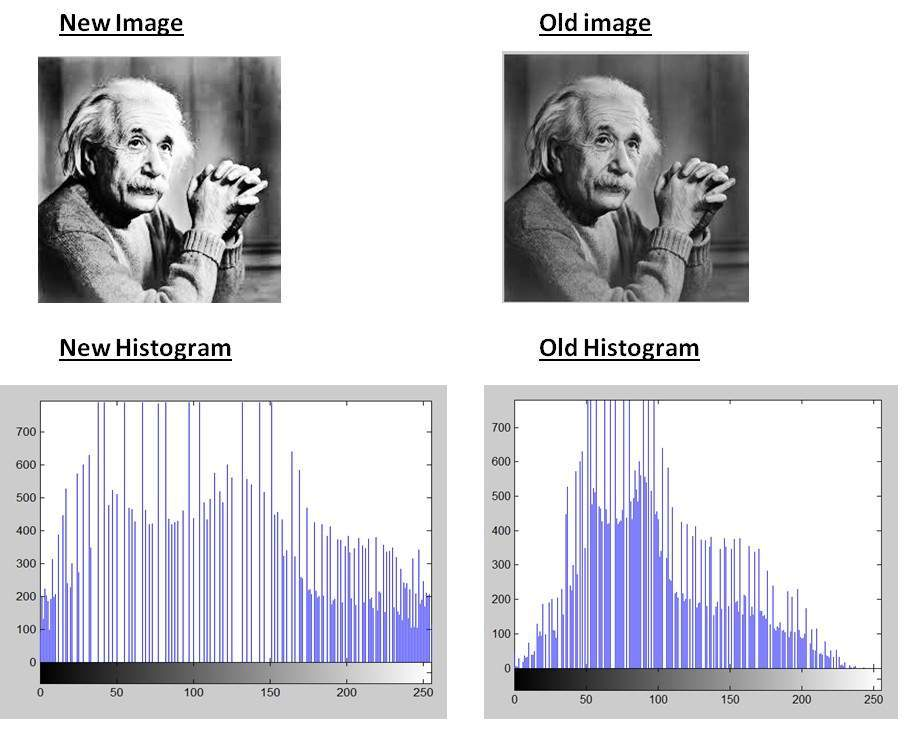
\includegraphics[width=\textwidth]{figures/histogram.jpg}
    \caption{A visualisation of histogram equalisation. On the right is the original image. On the left is the image after histogram equalisation. The histograms below the images shows how the contrast changes between the images. The histogram is stretched out where the bins are taller to ensure a better contrast between different pixel values.\cite{histogram}}
    \label{fig:contrast}
\end{figure}

The histogram equalisation calculates a cumulative histogram of an image which is a slope of the pixel values of the image. With the cumulative histogram, the areas with a steep slope, i.e. where the pixel value is appearing often in the image, can be used to determine a new grey-level mapping for the image. This is done by mapping the high density bins of the histogram to a wider interval of pixel values while mapping the low density bins to a narrower interval. This helps ensure a better contrast of the image, resulting in more reliable use of the Haar Classifier.\cite{imagebook}\\

Then, to perform the detection and classification of Haar-like features, OpenCV's \texttt{CascadeClassifier.detectMultiScale()} is used. With the features calculated, any face in the image should be detected.
The detection is done by applying different Haar-like features to the image to determine if any fit an area. If there is a positive match between the feature and the area, the cascade will continue trying different features to narrow down the area of a face. When an area of a face is narrowed down many different Haar-like features are compared to determine the match of a face. This can be seen in figure \ref{fig:Haar-featureFace}

\begin{figure}[H]
    \centering
    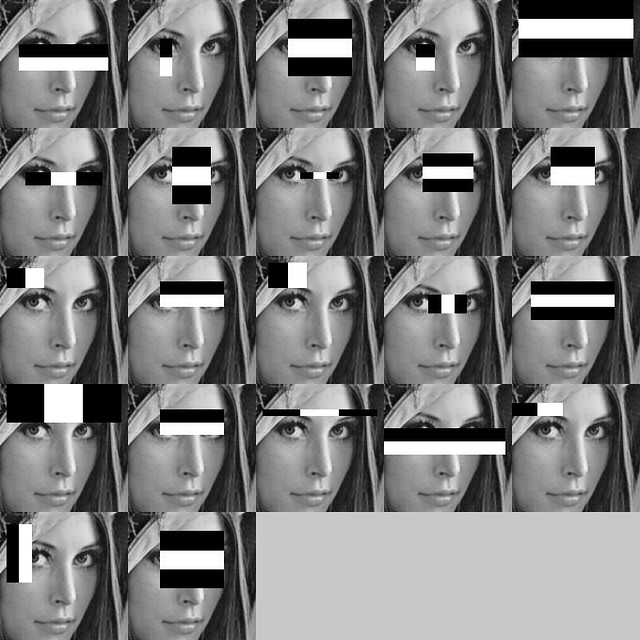
\includegraphics[width=0.8\textwidth]{figures/LenaHaarFeatures.jpg}
    \caption{The figure shows different Haar-like features applied to a face. These are applied at different stages to determine the presence of a face. If multiple features are not present the classifier will determine the likelihood of a face to be low and therefore, not classify it as such. In the figure both line features and edge features are shown.\cite{LenaHaarFeatures}}
    \label{fig:Haar-featureFace}
\end{figure}

The function detectmultiscale also gives a score the detected face in the image, there is also an adjustable value named neighbouring faces. The neighbouring faces is not how many faces is in the given image, when a face with Haar-cascade filter, as it is possible that a larger square or a shifted square has obtained the same image. The square with the larges scores is returned, meanwhile the other squares are considerate neighbouring faces.
\begin{figure}[H]
    \centering
    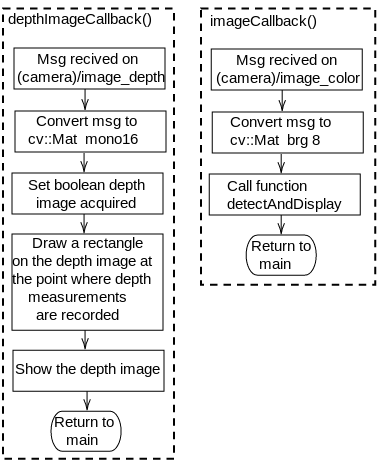
\includegraphics[width=0.6\textwidth]{figures/callback_face_flow.png}
    \caption{Flowchart of face and eye detection function implemented in this project. The two functions are described in there separate flowchart. The function detectAndDisplay and are described in flowchart later in this section, see figure \ref{fig:flowchartDetectface}}
    \label{fig:flowchartCallbacks}
\end{figure}


%Insert image of detected face


 With the detection of the face, the position of the face in the image is calculated. This can be used to determine the centre of the face for further use for detecting the position of the person as well as detect facial features. To further ensure that the detected face is indeed a face, eye detection is performed on the original image within the boundaries of the face previously calculated. The detection is done on the non-scaled image due to the size of eyes being too small in a down scaled image. Both the face- and the eye recognition can be seen on figure \ref{fig:detectedfaces}. 

\begin{figure}[H]
    \centering
    \begin{minipage}[b]{0.5\linewidth}
   Here two faces are detected and a circle is drawn from the centre of the face in pink, and the eye is drawn in the same fashion. Only one eye is detected, this is due to the high illumination of on the right side of the faces.\\
   About how the different callback functions work can be reviewed in figure \ref{fig:flowchartCallbacks}, and figure \ref{fig:flowchartDetectface}.
    \end{minipage}
    \hspace{0.2cm}
    \begin{minipage}[b]{0.47\linewidth}
    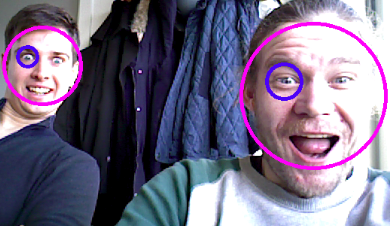
\includegraphics[width=\textwidth]{figures/detecedFace.png}
    \caption{The face- and eye detection, detecting two faces.}
    \label{fig:detectedfaces}
    \end{minipage}
\end{figure}



\begin{figure}[H]
    \centering
    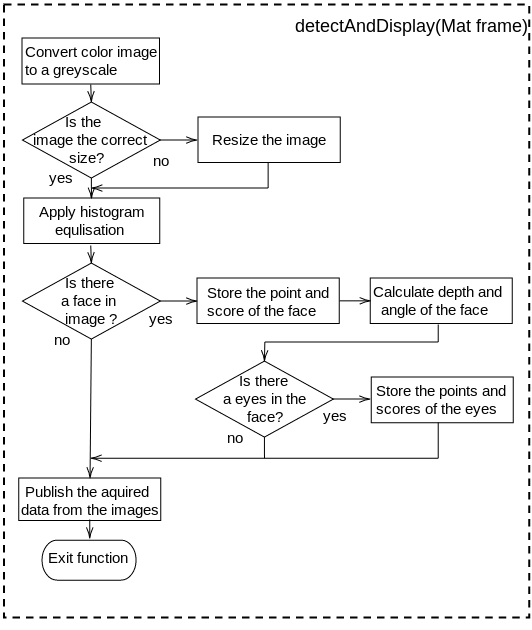
\includegraphics[width=0.8\textwidth]{figures/color_face_flow.png}
    \caption{Flowchart overview of the workings of the callback functions implemented in this project when a image message is received.}
    \label{fig:flowchartDetectface}
\end{figure}

With the face detected the position of the face in the image is used to extract the distance and angle to the person relative to the robot. The distance and angle are converted into an x and a y coordinate of the person. To see a visual representation of this, see figure \ref{fig:lidscan}. The angle is found by centre point of face in the detectmultiscale and maps the point between -1.0 and 1.0 and multiplied with the half width of cameras FOV in degrees
    

\begin{figure}[H]
    \centering
    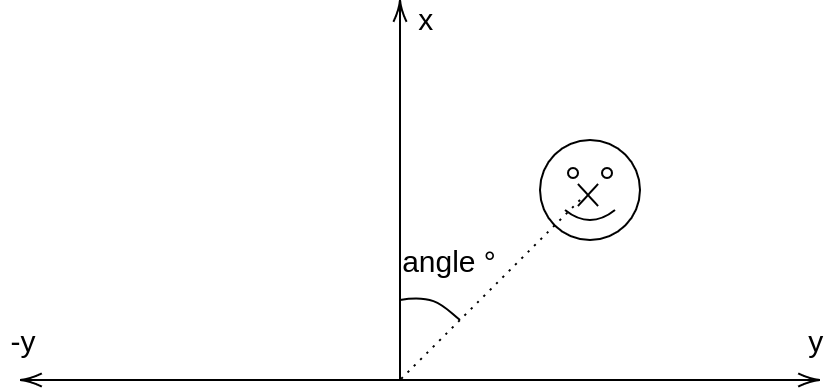
\includegraphics[width=0.7\textwidth]{figures/cameraview1.png}
    \caption{A visual representation of how the facedetector calculates the x-y coordinate of the persons tracked, where the dotted line is the length from the camera.}
    \label{fig:lidscan}
\end{figure}


Along with a ROS timestamp in the headers the xy coordinates is transmitted in a ROS-message to be used by the Kalman Filter for tracking of the person to be guided, described in section \ref{sec:KalmanFilter}.

The Kalman filter needs the covarince of the sensors. The covariance in this node is implemented as a variation over time, E.g the Cartesian xy coordinates is taken from each frame, that are captured of a person.
The mean or the sample mean which are implemented in this node, is because it is not possible to get a population mean, due to dropped data. 

The sample mean is calculated as so, where $\bar{x}$ is the sample mean of x.
\begin{equation}
    \bar{x} = \frac{1}{n-1} \times \sum_{n=1}^{25}x
    \label{eq:sampleXmean}
\end{equation}
\begin{equation}
    \bar{y} = \frac{1}{n-1} \times \sum_{n=1}^{25}y
    \label{eq:sampleYmean}
\end{equation}

From there the estimated variance of the x and y coordinates are calculated like so: where $\hat{\sigma_{x}}, \hat{\sigma_{y}}$ is the estimated sample variance
\begin{equation}
    \hat{\sigma^{2}_{x}} = (x - \bar{x}) \times (x - \bar{x})
    \label{eq:sigmaX}
\end{equation}
\begin{equation}
    \hat{\sigma^{2}_{y}} = (y - \bar{y}) \times (y - \bar{y})
    \label{eq:sigmaY}
\end{equation}

The estimated variance between y and x, also known as the covariance,
is calculated in the same manner with a slight difference.
\begin{equation}
    \hat{\sigma^{2}_{xy}} = (x - \bar{x}) \times (y - \bar{y})
    \label{eq:sigmaXY}
\end{equation}

Each calculation of the variance, $\sigma^{2}_{x}$ , $\sigma^{2}_{y}$and $\sigma^{2}_{xy}$, equations  \ref{eq:sigmaX},\ref{eq:sigmaY} and \ref{eq:sigmaXY} is based on the new x and y coordinate and sample mean.
The sample mean are calculated over a period of 25 frames, of the tracked person, an example can be seen in figure \ref{fig:varMean}. If only five frames has passed since the person is being tracked, the sample mean will only be calculated over the period of the five frames instead of 25 as seen in \ref{eq:sampleXmean}, \ref{eq:sampleYmean}. So there will be a period where the variance may fluctuate more than after the 25 frames are captured. Figure \ref{fig:varMean} depicts the implementation of the calculation of the variance.

\begin{figure}[H]
    \centering
    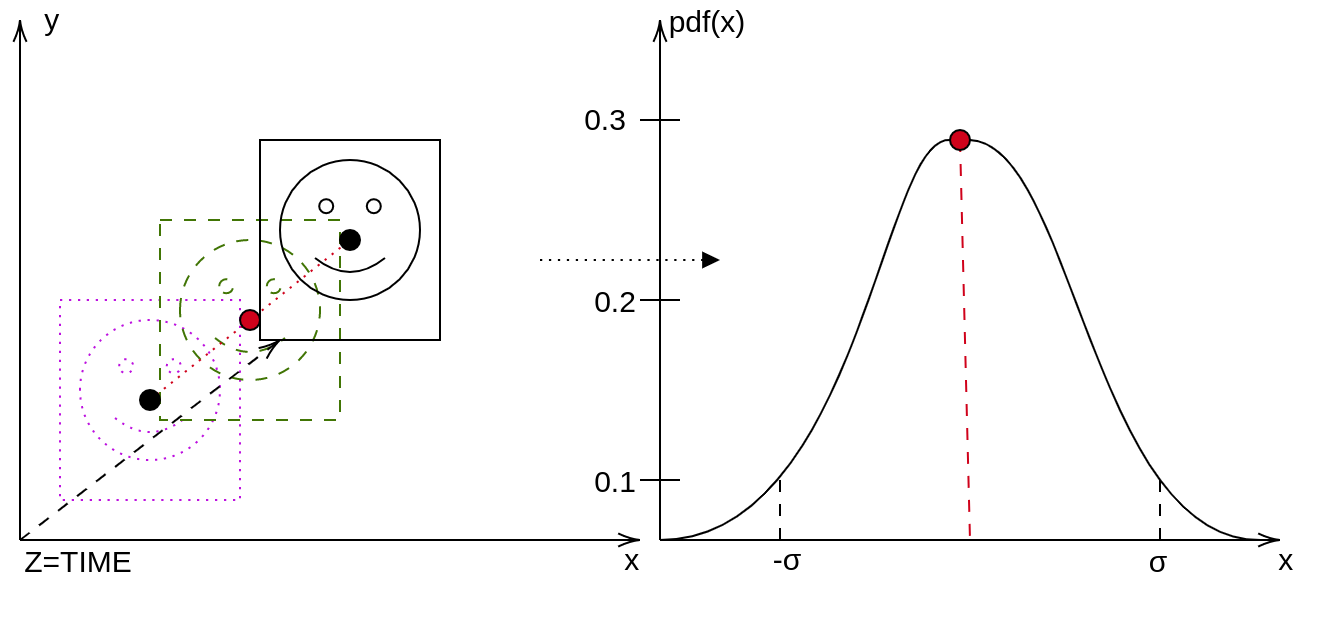
\includegraphics[width=\textwidth]{figures/mark2.png}
    \caption{This illustration of how the implementation of the variance of the xy coordinate. The face moves over time, the dots are the measured point of the persons, the red dot shall be seen as the average of the measurements, this is being translated to a variance in this example the variance of x. The $\sigma$ is the std. deviations, this can used to interpolate how far from the norm the measurement of x are.}
    \label{fig:varMean}
\end{figure}

%The face detector uses openCV to detect faces through stereo camera data. Haar-like features is used to get an initial set of detections, these features is based on change in contrast. A Haar group is formed if the detections line three or more adjacent pixels up with the necessary contrast values \cite{wilson2006facial}.
%The face detector then removes the false-positives by using the depth to predict the size of the head. Objects larger than the prediction will then be pruned.\\
%The face detector can be used as a continuous stream of data or as an action, where it will process the images until it has found at least one face. The action results is a list of faces found, the list is named face\_positions under people\_msgs/PositionMeasurement. It subscribes to the topic people\_tracker\_measurements, which contains the 3D position of the center of the face \cite{facedetect}.